\chapter{Material and Methods}
\chaptermark{\protect\parbox{.5\textwidth}{ARTICLE 1}}
\label{cap:linux}
\vspace{-2cm}

In this section, it is firstly described the dataset with emphasis in its composition, recovery of missing data and data transformation, important factors for the model accuracy. Secondly it is discussed the methodology for estimating potential evapotranspiration (PET), indispensable for calculus of water balance (TWB).
Lastly it is described the methodology used in the Artificial Neural Networks to forecast small spacial and temporal scales, that is the goal of this paper.

\section{Dataset}

The raw data used to establish the training set for the forecast model consists basically of the daily mean air temperature and the accumulated precipitation, these indexes were ground measured by conventional weather stations (CWS) and were the one available for this study.

It was chosen the most relevant agriculture production regions distributed in eight Brazilian states, in these locations it was selected ten CWS and its locations are shown in Table \ref{tab:locais}. 
The CWS were chosen based on geographical proximity of important agricultural centres and by its operation start date, the Fig.\ref{img:figure1} illustrates its distribution across Brazilian territory. The optimal range of data chosen for training the prediction model was from 1950 to 2011, the years of 2012 to middle 2015 were not known by algorithm for testing and validation purposes ensuring the learning and generalisation capacities of the artificial neural networks. The cross validation method adopted was the holdout method, which is basically a separation of the dataset in two sets, a training set and a validation set, that the function approximator tests its outputs with unknown data, given the large set of data this is an feasible validation method \cite{friedman2001elements}.

\begin{table}[ht]
  \centering
  \caption{Geographical locations of Brazilian ground-based conventional weather stations}
  \label{tab:locais}
  \begin{center}
  \begin{tabular}{llrrrr}
  \hline
  State & City & Maintainer & Lat(DD) & Long(DD) & Alt(m)\\
  \hline
  Paraná & Campo Mourão & INMET & - 24.05 & - 52.36 & 616.4\\
  Mato Grosso & Diamantino & INMET & - 14.40 & - 56.45 & 286.3\\
  Mato Grosso do Sul & Ivinhema & INMET & - 22.30 & - 53.81 & 369.2\\
  Ceará & Jaguaruana & INMET & - 4.78 & - 37.76 & 11.7\\
  Alagoas & Maceio & INMET & - 35.70 & - 64.50 & 64.5\\
  São Paulo & Presidente Prudente & INMET & - 22.11 & - 51.38 & 435.5\\
  & Jaboticabal & UNESP & -21.25 & -48.32 & 626.0\\
  & Piracicaba & USP & -22,73 & -47.64 & 547.0\\
  Goiás & Rio Verde & INMET & - 17.8 & - 50.91 & 774.6\\
  Minas Gerais & Uberaba & INMET & - 19.73 & - 47.95 & 737.0\\\hline
  
  \end{tabular}
  \end{center}
    
\end{table}

\begin{figure}[htb!]
\begin{center}
 \includegraphics[scale=0.5]{capitulo_2/w_s_location.eps}
 \caption{Weather stations locations}
 \label{img:figure1}
\end{center}
\end{figure}



There was air temperature measurements missing within all local datasets, a common problem in long time series. It was necessary to infill the gaps with estimated values to maintain consistency in the training processes.

\newpage
\section{Missing Data Recovery}
\label{sec:linux}

Traditionally the estimation of missing meteorological data are based on measurements of the same location, the reconstruction methods includes simple interpolations using mean values from time series arrays, or even using data from several days before and after the date with no measurement in a non-linear regression \cite{kim2010reconstructing}. ANNs are data-driven, non-linear statistical modelling tools capable to map and understand the relationship  between inputs and outputs, this ability renders it possible to simulate large-scale arbitrary complex linear problems \cite{wu2006flood} and are often used to forecast time-series \cite{zhang2003time, box1976time, french1992rainfall, zhang1998linear}.

The ANN implementation chosen was the feed-forward multilayer perceptron with one hidden layer and with 12 neurons, followed by a single neuron output layer. Time-series have a continuous nature and require a transfer function able to output a graded response, to meet this criteria it was chosen Logarithmic transfer function. The best performing transfer function was the logarithmic sigmoid (Eq. \ref{eq:solve}).

\begin{equation}
\label{eq:solve}
y = \frac{1}{1 + e^-x}
\end{equation}

Traditional backpropagation training algorithms are often too slow for practical problems. The performance of these algorithms are improved by allowing the learning rate to change during the training process and keep the learning step size as large as possible, while maintaining learning stable. Gradient search based technics such as backpropagation tend to get trapped at local minima, with enough gain (momentum) it can escape these local minima \cite{montana1989training}. To keep the algorithm responsive to the complexity of the local error surface while getting closer to the local minima, it was adopted the backpropagation with adaptive learning rate and momentum (GDX). The error function used in the ANN training processes was the mean squared error (MSE) represented by the following equation:
\begin{equation}
\label{eq:solve2}
MSE = \frac{1}{n} \sum\limits_{i=1}^n (\hat{Y}i - Yi)^2
\end{equation}
where \textit{n} is the length of the training array, \textit{\^{Y}}\textit{i} is the predicted value and \textit{Yi} is the observed value at an given time. 
All nodes weights were randomly initialised which was a problem, because of the non randomness of computer generated random numbers, this issue will be better
discussed further in the \textit{Binary Precipitation ANN} subsection. 

Normalising data can improve learning and can impact directly on the computational and classification performance \cite{shanker1996effect}. Prior beginning the training processes every place of the dataset were linearly transformed to the [0, 1] interval, being 0 the minimum value and 1 the maximum value of the dataset, this were done based on the Eq. \ref{eq:solve3}:
\begin{equation}
\label{eq:solve3}
Z_i^p = \frac{x_i^p - l_1}{u_i -l_i}
\end{equation}
where $Z_i^p$ is the transformed value, $l_i$ is the minimum and $u_i$ is the maximum value of the time series array. 

The dataset used to recover the lost air temperature, was the longest array without any missing air temperature for every location, in each subset it was left 
untouched around 20 percent of data for algorithm cross validation. It was made an correlation matrix to determine the time-space dependencies of the variable, being 
considered the interval dependent while the $\rho$ (Eq. \ref{eq:solve4}) value between the time-steps $x_{ij}$ and $y_{ij}$ was greater than 0.5, this was the
batch size for the entering layer for each ANN for this reason, it was different for every location.

\begin{equation}
\label{eq:solve4}
\rho = \frac{ \sum\limits_{ij=1}^n (x_{ij} - \bar{x})(y_{ij} - \bar{y})}{\sqrt{ \sum\limits_{ij=1}^n (x_{ij} - \bar{x})^2 \sum\limits_{ij=1}^n (y_{ij} - \bar{y})^2}}
\end{equation}

In the validation stage of these ANNs, the variance ($\sigma$) between the predicted value and the real one wasn't greater than 1 $^oC$ for every location, this was not the research goal and was considered reasonable to infill usage, no further validation was done and all gaps were filled.

\section{Weather Indexes Estimation}
\label{sec:linux}

The proposed model uses as input data based on estimated meteorological indexes which were the soil water content (SWC) in \textit{mm}, the daylight length in \textit{hours} and the extraterrestrial irradiation energy ($H_o$) in \textit{mm}. These indexes were chosen because of the inertia or carryover processes that they naturally have, these indexes are persistent and tends to have slightly changes from one observation to another unless some event such as precipitation happens. The theory is that the nested information which these indexes inherently carry are a important source of information for the ANN and an positive sign of the rainfall possibility.

To determine the SWC it is necessary to estimate the water balance. This is an practical method developed to quantify the water allocation among watersheds, which calculates its inputs and outputs sequentially, it is usually applied monthly but can be used for monitoring the soil water storage in near-real time \cite{thornthwaite1957instructions}, for the research it was used a daily scale.

In order to determine the water balance of a given place is necessary to estimate the potential evapotranspiration (PET). The PET is the amount of water to be evapotranspirated in a standard grassy surface if there was sufficient water available, this index is considered essential and represents the needed rainfall to supply the vegetation water needs \cite{de2000revisao}.

The PET values are usually estimated empirically by measured elements in weather stations, there are several methods to estimate its value. The choice of a method for estimating potential evapotranspiration depends on a number of factors. The first one is the availability of meteorological data, complex methods such as Penman–Monteith \cite{allen1998crop}, requires a great number of variables which are not aways available. Second is the temporal scale. Usually, empirical methods such as Thornthwaite, estimate the PET well on a monthly scale, whereas methods involving the radiation balance have a better performance in daily scale. Lastly, on empirical methods, it is required to know the climate conditions of which it were developed, some methods like Thornthwaite, are better for humid climates and not capable to perform on arid regions which requires different methods like the one proposed by Hargreaves and Samani \cite{hargreaves1985reference}.

The Thornthwaite method \cite{thornthwaite1948approach} was the first and widely know to estimate the PET value. It is a empirical method with the drawback of relying on the normal mean air temperature which is not aways available and to be created for humid regions. On 1971 Camargo\cite{camargo1971paulo} proposed an equation with practically the same results of Thorthwaite original work, without the drawback of needing normal air temperature and has the advantage of computing the extraterrestrial solar irradiation this method was analytically developed specifically for Brazilian conditions. This was the method adopted in this study, follows the Camargo equation:

\begin{equation}
\label{eq:solve9}
PET = 0.01 \,\, H_o \,\, Tn \,\, ND
\end{equation}
where $ND$ is the number of days contained in the desired period, $Tn$ is the period mean air temperature calculated in $^oC$ and $H_o$ calculated in ${MJ} \, m^{-2} \, day^{-1} $ is the extraterrestrial
irradiation energy falling on a plane horizontal to the earths surface throughout a whole day and is represented by the Eq. \ref{eq:solve10}:
\begin{equation}
\label{eq:solve10}
H_o = 37.6(1 + 0.033\cos(DOY\frac{360}{365}))[(\frac{\pi}{180^o}){N} \sin\phi \, \sin\delta + \cos\phi \, \cos\delta \, \sin P]
\end{equation}

In the $H_o$ equation \textit{DOY} represents the day of year, $\phi$ is the geographic latitude in \textit{degrees}, $\delta$ is solar declination calculated in \textit{degrees} 
based on Coopers\cite{cooper1969absorption} equation (Eq.\ref{eq:solve13}) and
\textit{N} is the photoperiod calculated in \textit{hours} by the equation \ref{eq:solve14}. The soil-moisture storage capacities was standardised in 100 \textit{mm} across all locations to simplify the calculus routine.

\begin{equation}
 \label{eq:solve13}
 \delta = 23.45 \sin[360 \, \frac{DOY - 80}{365}]
\end{equation}

\begin{equation}
\label{eq:solve14}
N = 2 \, \frac{\arccos[-\tan\phi \, \tan\delta]}{15^o} 
\end{equation}

With these estimated indexes, it was generated an new time-series dataset, for each Brazilian location, that were the estimated data used for the forecasting model with the addition of the the Unix time stamp for each day.

\section{Binary Precipitation ANN}
\label{sec:linux}

Traditionally in the field of modelling in climatology and time series, an auto regressive approach is used to solve the index forecasting problem \cite{rajurkar2002artificial, mishra2018rainfall, ramirez2006linear}. Rainfall is an sparse highly difficult to predict phenomenon that its occurrence depends on a series of complex parameters such as temperature, barometric pressure and wind speed \cite{sumi2012rainfall}. Given the nature this phenomenon these approaches relies on historical data that contains high variance, low bias and in short range period of times a great number of very small volumes or a lack of rainfall events. These characteristics make it difficult for traditional models to converge, which leads to a reduction of their potential performance.

The input selection is a key component to develop an accurate rainfall forecast model, many theoretical studies established the relationship between climate indices and rainfall.\citeauthor{tularam2010time} (\citeyear{tularam2010time}) showed an strong correlation in trend between rainfall and temperature ranges given the periodic nature of these variables.  \citeauthor{feng2016trend} (\citeyear{feng2016trend}) correlated water balance components such as PET with rainfall occurrence and proposed an annual rainfall ARIMA model with acceptable accuracy. \citeauthor{valipour2016much} (\citeyear{valipour2016much}) developed 3 models, for 4 climate conditions based on precipitation volumes capable of estimate monthly rainfall indices. \citeauthor{medvigy2012trends} (\citeyear{medvigy2012trends}) identified an strong correlation between increments of solar radiation and increases in precipitation variability. Despite the rationality and different exploratory methods on variables selection, studies have been approaching this issue taking in consideration the shortage of available and reliable data.

With this research it was intended forecast the rainfall occurrence in short periods of time with the premise that reducing the variance and rising the bias of the time series could lead to accuracy. To achieve this objective it was firstly determined the ranges of time that the model had to predict, which were from three to seven accumulated days. For each accumulated period it was generated an array containing the time-stamp of the last day of the period, the mean air temperature, the accumulated rainfall, an \textit{boolean} value to determine whether the accumulated precipitation was greater than 5\textit {mm} which is considered the median intensity of a light precipitation \cite{sun2006often}, the mean photoperiod, the soil water content and the average daily $H_o$, these were the final data that were used as inputs for for the ANNs and are represented by the following array representation:

\begin{table}[h]
 \caption{Inputs used for the ANN model}
\label{tab:netinputs}
\begin{center}
\begin{tabular}{ll}\hline
Data Name & Type\\\hline
Mean air temperature & $^oC$\\
Unix time stamp & \textit{datetime object}\\
Rainfall & \textit{mm}\\
Rainfall success flag & \textit{boolean}\\
Photoperiod & \textit{hours}\\
Water content & \textit{mm}\\
$H_o$ & \textit{mm}\\
\hline
\end{tabular}
\end{center}
\end{table}

With these new arrays was generated a new data array that were used to create four types of ANNs, one for each year climatic season based on the Unix time-stamp variable of the season change date.
Each type of ANN of each place is constituted of 5 ANN, one for every accumulated period($[3,...,7]$\textit{days}) consecutively each ANN had a well established rainfall pattern to predict.

To constraint even more the ANNs task, it was removed the necessity to predict the rainfall volume, by making as target for the model the boolean success flag. The goal with this methodology was to create a filter and in a future research, use as inputs only the time-steps that lead to rain,
limiting task of next ANN model, to predict only the amount of rain.

For each ANN the structure used was the multi-layer perceptron (MLP) feed forward, with backpropagation momentum and adaptive learning rate (GDX). The MLP structure usually consists of at least 3 layers, one input layer of which the receptors of the ANN receive external data, one output layer where the problem solution is obtained in this case whether or not it's going to rain. In the middle at least one intermediary layer called hidden layer with undetermined number of neurons, it was used a single hidden layer. To represents the structure a diagram of the ANN is shown in Fig. \ref{img:figure2} .

\begin{figure}[htb!]
 \centering
 
\includegraphics[scale=0.75]{capitulo_2/diagram_ann}
 \caption{Feedforward MLP structure}
 \label{img:figure2}
\end{figure}
The Mathematical structure of the feed forward multilayer perceptron with one output node can be represented by the following equation \cite{luk2000study}:
\begin{equation}
 \label{eq:solve15}
 y_1 = S_1(\sum\limits_{j=1}^{Nj} w_j S_2(\sum\limits_{i=1}^{Ni} w_i x_i))
\end{equation}

where $y_1$ is the output($[0, 1]$) of the network, $x_i$ is the input array (Fig. \ref{img:figure2}), $w_i$ the connection weights between the data node and the hidden layer, $w_j$ is the connection weights from the hidden layer to the output layer, $S_1$ is the activation function from the Input layer to the hidden layer, $S_2$ is the activation function from the hidden layer to the output layer.

One important decision in designing an backpropagation architecture is the selection of a proper activation function. The activation, or transfer functions are characterised by ruling the behaviour of output for each ANN node. They are a set of equations that have an limited amplitude and are the non linear transformation that is done over input signal \cite{karlik2011performance}. Sigmoid functions have a nonlinear nature and are widely implemented on backpropagation algorithms, they are easy to distinguish and can interestingly minimize the computation time for training and have an nonlinear output \cite{hecht1992theory, karlik2011performance}. Tangent sigmoid functions are a scaled version of a sigmoid function that solves the problem of values having the same signs. They have an steeper gradient with the advantage that that negative inputs will be mapped strongly negative and the zero inputs will be mapped near zero, this characteristics makes it suited for classification problems.

It was used two different activation functions, one tangent sigmoid (Eq.\ref{eq:solve11}) on $S_1$ and a hard limit (Eq.\ref{eq:solve12}) function on $S_2$. The reason for a hard limit transfer function was the definition of a binary target or an boolean value, in which the ANN would have only two forecasting possibilities.

\begin{equation}
\label{eq:solve11}
f(x) = \frac{\sinh{x}}{\cosh{x}}
\end{equation}
\begin{equation}
\label{eq:solve12}
f(x)=\begin{cases} 
      1 & \text{$if$ $x$ $>$ 0}\\
      0 & \text{$else$}
     \end{cases} 
\end{equation}

Determining the number of neurons in the hidden layer for a time-series problem is not an easy task \cite{zhang1998forecasting}, firstly the hidden layer of each ANN had 200 neurons,
then it was observed its forecasting accuracy and processing cost, then it was lowered to 50 without noticeable performance lost. With the results this was the number of neurons used and this parameter was not change in any of the ANNs in order to facilitate performance analysis and comparison.

The back propagation method is a technique used to update the nodes weights in supervised training ANNs. It is consisted of two passes throughout the different layers of the network, a forward pass and a backward pass. In the forward pass all the connection synaptic weights are fixed and a activity patterns is applied to the input nodes, then it propagates layer by layer, node by node producing a output signal as the network response. During the backward pass all the weights are corrected by an error-correction rule, that tries to minimize an error function, it was used the MSE (Eq. \ref{eq:solve2}), this is done by subtracting the actual ANN response by the desired response producing an error signal. All the network weights are backwardly adjusted to make the output closer to the desired one in a statistical sense \cite{dao2002performance}.

At the first learning epoch of the ANNs the first weights has to be randomly distributed within the $[0, 1]$ limits, this first random distribution was a problem. The computer is a deterministic machine and to generate random numbers by a deterministic machine a pseudo random number generator is needed. A random generator is an algorithm that produces numbers or vectors that its properties approximates of truly random numbers, this algorithm usually has a seed parameter that uses the computer clock, which can lead to an normal distribution of the random numbers, for this reason sometimes it was required to run the training processes several times. After the first weights distribution, the equation that defines the weights adjustment for each iteration $w_{n + 1}$ of the algorithm was:

\begin{equation}
 \label{eq:solve16}
w_{n+1} = w_n - \alpha_{n + 1} \,\, g_n + \mu \,\, w_{k - 1}
\end{equation}

where $g_n$ is the gradient of the error to the weight vector, $\alpha$ is the learning rate and $\mu$ is the momentum constant. The momentum term is used to avoid the weight adjustment to be
stuck in the local minima and reduce the algorithm instability \cite{haykin2004comprehensive}, the $\mu$ value must be variate between 0 and 1 but it is recommended to use values between 0.4 and 0.9 \cite{wythoff1993backpropagation}.
An low $\mu$ value increases the risk to the ANN get stuck in the local minima and a excessively high value might make the model surpass the problem solution, it was used for all the ANNs an value of 0.9.

Other particularity of the model, despite the back propagation and the $\mu$ constant, was the use of variable learning rate, the learning rate is a parameter used in the back propagation stage to define the conversion speed to the minimum solution. Setting the \textit{lr} too high the algorithm would converge too fast making it unstable, setting too low would make it to take too long to find the minimum solution or even never find it. To optimize the forecasting problem, the ANN uses an larger $\alpha$ when it 
is far from the solution and progressively decreases it while it gets closer by the use of the Eq. \ref{eq:solve17} and Eq. \ref{eq:solve18}.

\begin{equation}
\label{eq:solve17}
\alpha_{n + 1} = \beta \, \alpha
\end{equation}

\begin{equation}
\label{eq:solve18}ht
\beta = \begin{cases}
         0.7 & \text{$if$ $\frac{error_n}{error_{n-1}}$ $>$ 1.04}\\
         1.05 & \text{$if$ $\frac{error_n}{error_{n-1}}$ $<$ 1.04}
        \end{cases}
\end{equation}

Having been determined the basic ANNs structure, we had to choose how many steps before should be appended in each input array to be computed by the ANN to forecast one step further or $t + 1$,
which were call by time-steps, these time-steps are the amount of lagged arrays (Fig. \ref{img:figure2}) that should be used as inputs for the ANNs, this concept is shown in the Fig. \ref{img:figure3} which represents one time-step array,  two time-steps array, up to the time-series length (\textit{n time-steps}). To optimize the lag determination it was made an correlation analysis, for each place and accumulated period, just as in the time-series missing data recovery, that was done autonomously by the algorithm and was set to select only an number of time-steps that had an $\rho$  value bigger than 0.5. This time-step parameter ranged from $t-1$ in the least correlated vectors up to $t-4$ in the most correlated vectors.

\begin{figure}[htb!]
 \centering
 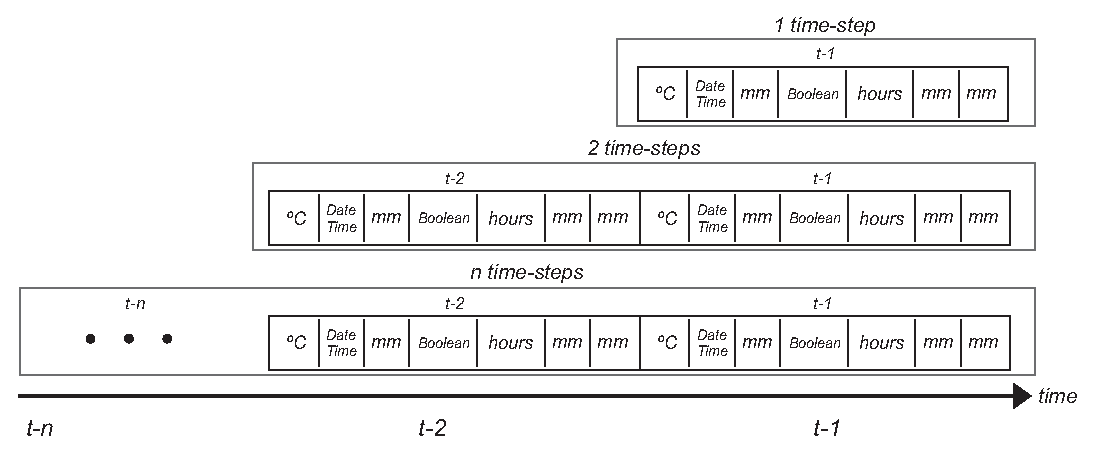
\includegraphics[scale=0.88]{capitulo_2/time_steps}
 \caption{Diagram of the time-steps concept }
 \label{img:figure3}
\end{figure}

\newpage

ANNs training become more efficient if certain preprocessing steps are made on data. Normalisation is crucial to prepare data to made it suitable for training, without this step training would be slow and ineffective. In order to minimize bias into each input feature that have widely different scales, this process is made to scale down data into a similar range \cite{yaldi2009improving}. There are many types of normalisation procedures such as statistical normalisation, that produces data where each feature has a zero mean and a unit variance and Min-Max normalisation that rescales features from one range to a new one depending on the type of activation function    

To keep data inside the constraints of the tangent sigmoid transfer, fitting it into the $[-1, 1]$ interval and making it proper for training, the dataset was normalised by the Min-Max normalisation method demonstrated by the Eq. \ref{eq:solve19}. Then the algorithm was set to run and train all the ANNs models. It was generated 200 individual rainfall forecasting ANNs based on the described methodology, the results of this research are the accuracy of each individual ANN.

\begin{equation}
 \label{eq:solve19}
 Z_i^p = -((\frac{-2(u_i - x_i^p)}{u_i - l_i}) + 1)
\end{equation}

%%\begin{figure}[htbp]
%\begin{figure}[H]
%\tiny \caption{\small Ilustração do sistema operacional como interface entre o usuário e os recursos do sistema. \label{S.O.}}
%% o que está dentro do colchetes é o que aparecerá na lista de figuras.
%\vspace{-0.3 cm}
%\begin{center}
%\begin{psfrags}
%\epsfxsize=4cm
%\centerline{
\includegraphics[width=4.0 cm]{./capitulo_2/tux-linux.eps}}
%\end{psfrags}
%{\small Fonte: Adaptado de \citeonline{llgarver_sept70}}
%\end{center}
%\end{figure}
%
%\newpage % para passar o exemplo de citação para a próxima página.

